% Template for APA submission with R Markdown

% Stuff changed from PLOS Template
\documentclass[a4paper,man,apacite,floatsintext]{apa6}
\usepackage{apacite}

% amsmath package, useful for mathematical formulas
\usepackage{amsmath}
% amssymb package, useful for mathematical symbols
\usepackage{amssymb}

% hyperref package, useful for hyperlinks
\usepackage{hyperref}

% graphicx package, useful for including eps and pdf graphics
% include graphics with the command \includegraphics
\usepackage{graphicx}

% Sweave(-like)
\usepackage{fancyvrb}
\DefineVerbatimEnvironment{Sinput}{Verbatim}{fontshape=sl}
\DefineVerbatimEnvironment{Soutput}{Verbatim}{}
\DefineVerbatimEnvironment{Scode}{Verbatim}{fontshape=sl}
\newenvironment{Schunk}{}{}
\DefineVerbatimEnvironment{Code}{Verbatim}{}
\DefineVerbatimEnvironment{CodeInput}{Verbatim}{fontshape=sl}
\DefineVerbatimEnvironment{CodeOutput}{Verbatim}{}
\newenvironment{CodeChunk}{}{}

% cite package, to clean up citations in the main text. Do not remove.
\usepackage{cite}

\usepackage{color}

% Use doublespacing - comment out for single spacing
%\usepackage{setspace}
%\doublespacing


% Text layout
\topmargin 0.0cm
\oddsidemargin 0.5cm
\evensidemargin 0.5cm
\textwidth 16cm
\textheight 21cm

% Bold the 'Figure #' in the caption and separate it with a period
% Captions will be left justified
\usepackage[labelfont=bf,labelsep=period,justification=raggedright]{caption}


% Remove brackets from numbering in List of References
\makeatletter
\renewcommand{\@biblabel}[1]{\quad#1.}
\makeatother


% Leave date blank
\date{}

%\pagestyle{myheadings}
%% ** EDIT HERE **


%% ** EDIT HERE **
%% PLEASE INCLUDE ALL MACROS BELOW

%% END MACROS SECTION


% ALL OF THE TITLE PAGE INFORMATION IS SPECIFIED IN THE YAML
\title{\textbf{Children's Processing of Ad-hoc Implicatures: Measuring Developmental
Gains in the Speed and Accuracy}}
\shorttitle{Children's ad-hoc implicature processing}

\author{Erica J. Yoon, Michael C. Frank}

\affiliation{Department of Psychology, Stanford University}

\authornote{}
\abstract{Language comprehenders routinely make pragmatic inferences that go
beyond the literal meanings of utterances. If A said ``I ate some of the
cookies,'' B should infer that A ate some \emph{but not all}. Children
perform poorly on experimental tests of scalar implicatures like this,
despite their early-emerging sensitivity to pragmatic cues. Children
have been more successful with ad-hoc (contextual) implicatures (e.g.~In
a context with two faces, a face with only glasses and a face with
glasses and a top-hat, \emph{My friend has glasses} is more likely to
refer to face with only glasses; Stiller, Goodman, \& Frank, 2015).
Using simplified tasks that measure both speed and accuracy of ad-hoc
implicature processing, our current work explores potential factors
responsible for children's successes and failures in computing
inferences. In three experiments, we used an eye-tracking paradigm
(Experiments 1 and 2) and a tablet paradigm (Experiment 3) to test
children's ability to compute implicatures when they have access to
contextual alternatives to the target word. The findings suggest that
children as young as three years old can successfully identify target
referents of ad-hoc implicatures. We also found some evidence that
salience of distractor is a potential cause of children's struggle with
implicature computation in our task. Our work contributes to the growing
literature of early signs of pragmatic understanding in children.}
\keywords{Pragmatics; cognitive development; implicature; inhibitory demand;
eye-tracking; tablet}

\begin{document}
\maketitle

\section{Introduction}\label{introduction}

Language comprehension involves not only interpreting the literal
meanings of words in utterances, but also inferring intended meanings
behind what is said. Imagine that Bob bought two kinds of cookies to
eat, chocolate-chip and raisin, and left them on a table. Alice
approaches and says to Bob, ``I ate some of your cookies, the
chocolate-chip ones.'' Later, Bob is surprised to find that Alice ate
all of his cookies, chocolate-chip and raisin. If it is technically true
that Alice ate some (i.e.~one or more) cookies, and chocolate-chip
(alongside raisin) cookies, why would Bob be surprised that Alice ate
all the cookies?

Communication is a cooperative act, and when people fail to meet this
expectation, misunderstandings arise. According to Grice (1975), people
tend to ``make their contribution as required, when it is required, by
the conversation in which they are engaged,'' thereby being maximally
informative. In the previous scenario, Alice was not as informative as
she could be by saying she ate \emph{all} of the cookies, and thus led
to Bob's misunderstanding that Alice ate some of the cookies \emph{but
not all}. Alice thus failed to warn against the assumption that she was
making \emph{pragmatic implicature}, where speaker's implied meaning
goes beyond the literal meaning of the utterance.

Pragmatic implicatures are important for proficient language use, as
they are common and efficient ways of implicitly expressing speakers'
intended meanings. For example, if a child asks a parent whether they
could have cookies for snack, and a parent says: ``you can have some of
the cookies,'' the child should be able to infer that she should eat
some but not all of the cookies. Thus, implicatures would make up an
important case study for adults' and children's pragmatic understanding
and show what they can infer about speaker's implicit communicative
intentions.

Whereas adults robustly process implicatures, studies have shown mixed
results about children's ability to compute implicatures, and it is not
yet clear what cause children's successes and failures in implicature
computation. In the next section, we review previous research on
children's processing of implicatures.

\subsection{Previous work on preschoolers' implicature
computation}\label{previous-work-on-preschoolers-implicature-computation}

Research on children's implicature processing has mainly looked at
processing of \emph{scalar} implicatures and \emph{ad-hoc} (contextual)
implicatures. In the previous example of Alice's utterance, ``I ate some
of the cookies'' is a scalar implicature (\emph{SI}): it implicates that
she ate some but not all, which relies on generating the relevant
lexical scale upon hearing the weaker term ``some'' (Horn, 1972) and
negating the stronger alternative (``all''). On the other hand, ``I ate
chocolate-chip cookies'' is an example of contextual or ad-hoc
implicature, which involve the knowledge of contextually-derived scales
or alternatives: in this example, use of the contextually weaker term
(``chocolate-chip cookies'') negated the stronger description
(``chocolate-chip and raisin cookies).

While adults are successful at computing SI's, children largely
struggle. Adults readily compute scalar implicatures, even though
implicature inferences are generally slower than processing of
unambiguous meanings (Bott \& Noveck, 2004; Grodner, Klein, Carbary, \&
Tanenhaus, 2010; Huang \& Snedeker, 2009a) However, numerous studies
have reported that children seem to have difficulty computing SI's for
scalar contrasts between words such as \emph{might} vs. \emph{want},
\emph{some} vs. \emph{all}, and \emph{or} vs. \emph{and} (Chierchia,
Crain, Guasti, Gualmini, \& Meroni, 2001; Gualmini, Crain, Meroni,
Chierchia, \& Guasti, 2001; Huang \& Snedeker, 2009b; Noveck, 2001;
Papafragou \& Musolino, 2003). For example, Papafragou \& Musolino
(2003) presented adults and 5-year-old children with a context in which
three out of three horses jumped over a fence. Then a puppet offered a
description of the context by saying: ``some of the horses jumped over
the fence.''' When asked whether what the puppet said was a good
description of what happened, most of the adults denied it, whereas
almost 90\% of the children accepted it as an adequate description.

A real-time eye-tracking paradigm also revealed that children fail to
identify the correct target of SI. Huang \& Snedeker (2009b) presented
two girls and two boys, for example, and girl A had two socks, boy B
also had two socks, girl C had three soccer balls and boy D had none of
the items. Based on this context, girl A had two out of four, hence
``some but not all'' of the socks, whereas girl C had three out of
three, or ``some and indeed all'' of the soccer balls. Hence, it was
predicted that, if children computed the implicature ``some but not
all,'' then children would look immediately toward the girl with socks
rather than the girl with soccer balls upon hearing ``some.'' However,
children did not look to the correct target above chance until after the
disambiguation phase (i.e., between ``socks'' vs. ``soccer balls'').

Whereas preschoolers struggle with SI computation, they have shown more
promising performances on \emph{ad-hoc} implicature tasks. Since ad-hoc
implicatures are based on contextual scales, tasks using ad-hoc
implicature can easily provide visual access to alternatives
(e.g.~chocolate-chip cookies versus chocolate-chip \emph{and} raisin
cookies), thereby reducing the difficulty for children to spontaneously
generate relevant alternatives to the term offered.

Papafragou \& Tantalou (2004) showed that, in a context where a puppet
was instructed to e.g., wrap two gifts (a parrot and a doll), and he was
asked ``Did you wrap the gifts,'' 4- to 6-year-olds correctly rejected
to reward the puppet who said, ``I wrapped the parrot.'' Based on these
results, Papafragou and Tantalou claimed that children were able to
compute implicatures and when the constitution of alternatives (parrot
vs.~parrot and doll) was possible. Barner, Brooks, \& Bale (2011) also
showed that 5-year-olds, who saw three out of three animals (a cat, cow,
and dog) sleeping, correctly reject the statement ``only cat and cow are
sleeping'' but not ``only some of the animals are sleeping,'' again
showing that access to alternatives may be crucial for children. Katsos
\& Bishop (2011) found additional evidence that 5-year-olds can compute
ad-hoc implicatures, as they gave lower reward for under-informative
utterances with ad-hoc scales (e.g. ``The dog painted the triangle,''
implicature: ``but not the star'').

Stiller, Goodman, \& Frank (2015) provided evidence of successful ad-hoc
implicature computation in that children 3.5 years and above, youngest
to date to show ability to make implicatures. They presented 2- to
4-year-old children with pictures of three different faces, for
instance: one wearing glasses and a top hat, another one wearing only
glasses, and another wearing none of the two. Then a puppet said, ``my
friend has glasses,'' then asked children to pick out the correct
referent. Given the context, only using the term ``glasses'' implicates
the referent has ``glasses but not a top-hat,'' suggesting that the face
with only glasses is the referent. Indeed, Stiller et al. found that
children as young as 3.5 years of age chose the implicature-consistent,
one-feature referent above chance when they heard utterances such as
``my friend has glasses.''

In sum, children struggle on SI computation tasks, but children of 4
years of age and above successfully compute ad-hoc implicatures.
However, commonly across all previous research, children younger than 3
years consistently fail. In the next section, we explore possible causes
of younger children's struggle with implicatures.

\subsection{Younger children's struggle with implicature
computation}\label{younger-childrens-struggle-with-implicature-computation}

What causes younger children to fail on implicature tasks? One
possibility is children younger than 2 years do not yet have
well-established pragmatic understanding. However, this explanation
seems unlikely given children's early-emerging sensitivity to
informativeness of utterances, an important skill for implicature
computation and general pragmatic understanding. Children are adept at
sensing informativeness of others' and their own utterances: at two
years of age, children start to adjust informativeness of their own
expressions depending on the listeners' knowledge by 3 years of age
(Matthews, Butcher, Lieven, \& Tomasello, 2012; Matthews, Lieven,
Theakston, \& Tomasello, 2006) and assess informativeness of their own
gestures (O'Neill \& Topolovec, 2001). Thus, even young children seem to
excel at assessing the informativeness of both their own and other
people's utterances and communicative gestures, which suggests that lack
of general pragmatic understanding is not the cause of their failures on
SI computation.

Another candidate for younger children's difficulty is inhibitory
control, more specifically their inability to restrain choosing or
directing their attention to more salient referents. For example, many
of the experimental tasks on implicature computation required children
to reject potential referents that represent stronger alternative than
the term offered to them. These distractors were often more salient for
having more features (a face with ``glasses and top-hat'' versus a face
with only ``glasses''), and may have been harder to draw attention away
from.

This ``inhibitory hypothesis''" is in line with predictions from other
relevant developmental findings. The effects of salience show up in
other findings of pragmatic development, including younger children's
word learning (Yurovsky \& Frank, 2015). Research on children's
executive functions report that younger children have difficulty with
executive control, and the ability for inhibitory control continues to
develop throughout childhood (Davidson, Amso, Anderson, \& Diamond,
2006; Diamond \& Taylor, 1996).

One way to test the inhibitory hypothesis would be to manipulate
salience of the distractor to see if children's attention is drawn away
from the target toward the distractor. This approach gives rise to
interesting predictions for tradeoffs between inhibitory demand and
pragmatic computation. On one hand, inhibitory hypothesis predicts that
as salience contrast increases (i.e.~distractor becomes much more
salient than the target with more features: face with glasses (target)
vs.~face with glasses, top-hat, \emph{and bow tie}), it will be more
difficult for children to direct their attention to the inferential
target that is less salient. On the other hand, however, Gricean
communicative principle and computational model of pragmatic inferences
(Frank \& Goodman, 2012) suggest that the increased contrast strengthens
the implicature in question: it is more informative to say ``My friend
has glasses'' to refer to the face with only glasses in a context where
there is another face with an extra feature (face with glasses and
top-hat), and even more informative in a context with a face with
\emph{two} extra features (face with glasses, top-hat, and bow tie).
Thus, as the salience of the distractor increases, the inhibitory demand
would favor the distractor, but the pragmatic computation would favor
the target, and it will depend on whether children rely more on one or
the other aspect of the task.

\subsection{The current study}\label{the-current-study}

To confirm preschoolers' ability to compute implicatures and explore
potential causes of younger children's struggle, we present a set of
studies that take a closer look at children's implicature processing
abilities. The goals of the current studies were (1) to confirm that
children robustly compute ad-hoc implicatures starting at an early age
(3-4 years); and (2) to identify what causes younger children's struggle
with implicature computation. To do this, we need a measure of not only
\emph{what} children choose as their final answer in implicature task
but also \emph{how}. For example, reaction time is a measure that allows
a closer look at children's inferential decision-making process, but
many previous studies lacked this measure.

Thus, here we implement two different methodological tools to look at
timecourse and speed of implicature processing: eye-tracking and tablet
paradigms. Eye-tracking is a useful tool for looking at real-time
inferential decision-making process, and may help identify factors that
contribute to how much fast decisions are made, and how much attention
is allocated to each potential referent, depending on utterances and
contexts. Tablets provide an engaging way to collect data from young
children, and is useful in that it yields comparable data to that of
behavioral paradigms, while making it possible to examine the accuracy
and speed (reaction time) of children's judgments (Frank, Sugarman,
Horowitz, Lewis, \& Yurovsky, 2016). These two tools can complement each
other in their strengths as naturalistic and engaging methods that
reveal time-sensitive information about children's implicature
processing.

In Experiment 1, we used an eye-tracking paradigm with a simplified
design to test children's ability to compute ad-hoc implicatures:
children saw two items with single or double features (e.g., a plate
with a carrot and banana, and a plate with only a carrot) and heard the
common feature (e.g., carrot) named, suggesting an implicature (i.e., a
carrot but not a banana). We identify one potential factor that
contributes to children's implicature processing: salience-pragmatic
tradeoff, or tradeoff between perceptual salience versus strength of
implicature. In Experiment 2 and 3, we explore the effect of
salience-pragmatic tradeoff, using eye-tracking (Experiment 2) and
tablet paradigm (Experiment 3). We find that children as young as 3
years of age robustly compute ad-hoc implicatures in our paradigm, and
we report some evidence for salience affecting young children
(2-year-olds)'s implicature computation performance.

\section{Experiment 1}\label{experiment-1}

In Experiment 1, we use an eye-tracking paradigm to look at children's
ad-hoc implicature computation. As previously mentioned, A previous
eye-tracking paradigm looking at SI computation in children Huang \&
Snedeker (2009b) suggested that children do not calculate SI during
online language processing. However, children might have struggled with
SI computation from the lack of access to lexical scales (some-all), and
the time constraint to process implicatures (in less than one second).
Our current work uses a similar but simpler paradigm that tests
children's inference of implicatures given scales that are set up
contextually.

Thus, in addition to replicating previous research on ad-hoc
implicatures in the online processing context, we are able to pursue two
goals in Experiment 1: measure the time-course of ad-hoc pragmatic
inference; and identify potential factors that contribute to the
developmental differences in implicature computation performance.

\subsection{Method}\label{method}

\subsubsection{Participants}\label{participants}

Parents and their 2- to 5-year-old children visiting Children's
Discovery Museum in San Jose, CA, were invited to participate in a short
video study. A total of 150 children were recruited but a few were
excluded from the sample for the following reasons: age other than 2 to
5 years (n = 11), parent-reported English exposure less than our
prespecified criterion of 75\% (n = 11), noncompliance or difficulty
with the experimental procedure (n = 7), experimenter error or technical
issues (n = 4). In addition, individual trials with more than 40\%
missing gaze data were excluded from analysis, and only participants who
completed at least 60\% of the trials (10 out of 16) according to this
criterion were included in the analysis. These exclusion criteria led to
a final sample of 117 (out of 127 participants who qualified; see Table
1). Children were given a sticker for participating in the study. We
also tested fourteen adult participants, undergraduate students
recruited through Stanford Psychology credit pool.

\begin{table}[tb]
\centering
\begin{tabular}{lccccc}
  & Age bin & Mean (years) & Participants & Girls & Proportion kept \\ 
  \hline
Expt 1 & 2 & 2.6 & 27 & 9 & 0.93 \\ 
    & 3 & 3.5 & 33 & 21 & 0.94 \\ 
    & 4 & 4.5 & 29 & 14 & 1.00 \\ 
    & 5 & 5.4 & 34 & 15 & 1.00 \\ 
  Expt 2 & 2 & 2.6 & 28 & 16 & 0.97 \\ 
    & 3 & 3.5 & 21 & 10 & 0.91 \\ 
    & 4 & 4.4 & 30 & 15 & 1.00 \\ 
    & 5 & 5.5 & 23 & 9 & 0.88 \\ 
  Expt 3 & 2 & 2.5 & 25 & 18 & 0.86 \\ 
    & 3 & 3.5 & 29 & 16 & 0.97 \\ 
    & 4 & 4.4 & 25 & 8 & 0.96 \\ 
    & 5 & 5.3 & 19 & 11 & 1.00 \\ 
   \hline
\end{tabular}
\caption{Demographic information of participants in Experiments 1 and 2, and proportion of participants who are qualified and complete the study that are included in the analyses.} 
\label{tab:exp1_summary}
\end{table}

\subsubsection{Stimuli and Design}\label{stimuli-and-design}

On each trial, participants saw two images: a target and distractor,
which could either be an item with a single feature (e.g.~a plate with
only a carrot or only a banana), or an item with double features (e.g.,
a plate with a carrot and a banana). Each trial contained three phases:
in the initial phase (8.5 seconds), two images were presented in silence
for two seconds, then a pre-recorded voice said a sentence (e.g. ``Look
at these plates. Elmo's plate has a carrot.''). Then, in the
anticipatory phase (1.5 seconds), a chime sound played to induce
participants' anticipatory gaze. In the following feedback phase (1.5
seconds), a character appeared next to the target with an amusing sound
effect. This outcome served to keep the task engaging for participants.

There were three types of test trials (shown in Figure 1). In
\emph{inference} trials, the target item had a single feature (e.g., a
carrot), and the distractor item had two features, one that was common
with the target (e.g., a carrot) and the other feature that was unique
(e.g., a banana). The test sentence named the feature that was common to
the target and distractor. Thus, if participants understood that
``Elmo's plate has a carrot'' implicates ``Elmo's plate has a carrot
\emph{but not a banana},'' given the context, they should look more
toward the target than the distractor, but otherwise look equally to
both.

There were two additional trial types, with semantically unambiguous
targets: \emph{Control-double} trials looked identical to inference
trials, but the target and distractor were switched, such that the
double-feature item was the target and the single-feature item was the
distractor, and the test sentence named the unique feature on the
target. \emph{Control-single} trials presented two items that each had a
unique single feature, and either could be the target. Children saw 4
inference, 4 control-double, and 4 control-single trials; adults saw 6
inference, 6 control-double, and 12 control-single trials.

There were six sets of item and feature types, and the features were
named with nouns found on the MacArthur-Bates Communicative Development
Inventory word list (Fenson et al., 1994). Two orders of the test trials
were created, such that trial types and item types were counterbalanced
and trial order was pseudo-randomized across the two orders.

\subsubsection{Procedure}\label{procedure}

Participants sat in a booster seat, approx. 60 cm away from the monitor
of an SMI RED 120 Hz binocular remote eye-tracker. Participants were
introduced to the task as watching a short video. The video began with a
short Elmo video clip that lasted for 1-2 minutes, during which any
necessary adjustments to the eye-tracker and participants' chair
positions were made. The eye-tracker was then calibrated using a 2-point
calibration and validation of the calibration points. Then participants
were introduced to Sesame Street characters and told ``Today, {[}they{]}
will show us lots of fun things. Are you ready? Let's go!'' Following
the introduction, participants saw two gaze-contingent practice trials,
with unambiguous targets that differed from the test items. Then
children watched 16 test trials and adults watched 24 test trials, as
well as 4 filler photos of children playing and 2 Elmo video clips,
presented at a pseudo-random points between test trials. The video
lasted approximately 8 minutes.

\subsection{Results and Discussion}\label{results-and-discussion}

\begin{CodeChunk}
\begin{figure}[H]

{\centering 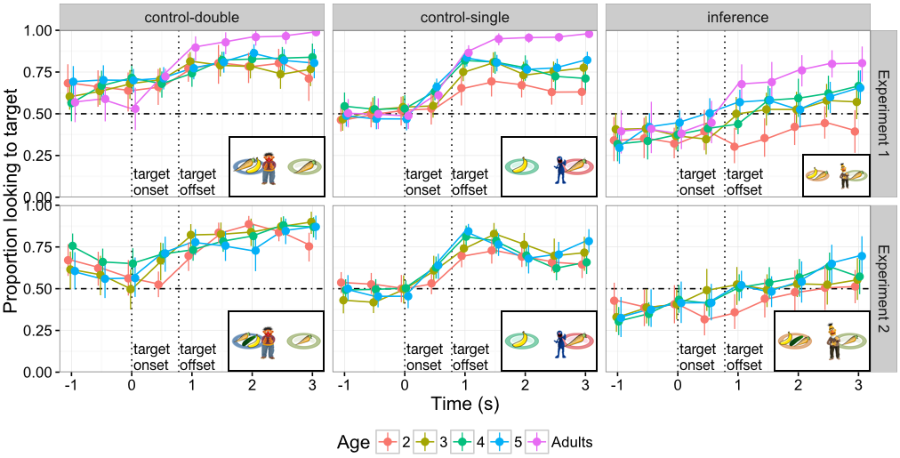
\includegraphics{figs/et_acc-1} 

}

\caption[Proportion of 2- to 5-year-old children and adults looking to the target image as the utterance unfolds in Experiments 1 and 2 (rows), in different trial types (columns)]{Proportion of 2- to 5-year-old children and adults looking to the target image as the utterance unfolds in Experiments 1 and 2 (rows), in different trial types (columns). Time 0 represents the target word onset, and time 0.78 represents the average target word offset. Proportion correct looking is defined by looks to the target divided by the total looks to both the target and the distractor. Example stimuli are shown in the bottom right hand corner for each condition; the named character emerged at the end of the trial to mark the correct target.}\label{fig:et_acc}
\end{figure}
\end{CodeChunk}

Participants of all ages looked to the targets in both control-double
and control-single trials reliably above chance (50\%; Figure 1). There
were age differences in the speed of looking at the target and the
proportion of correct looking across both control trial types.

For inference trials, children of 4 years and above robustly looked to
inferential targets (for 4-year-olds: \(t\)(28) = 2.55, \(p\) =0.016).
For example, upon hearing ``Bert's plate has a carrot,'' older children
identified the plate with only a carrot as the referent rather than the
plate with a carrot and a banana, replicating Stiller et al. (2015)'s
findings of ad-hoc implicature. Although previous studies are not
directly comparable due to low-level differences in the task and
materials, our finding is consistent with the hypothesis that children's
inferential ability might have been obscured in previous SI tasks due to
the unavailability of lexical alternatives (e.g. ``all'' given ``some'';
Barner et al. (2011)).

We additionally observed an unpredicted trend in two-year-olds'
behavior: they did not disengage from distractors relative to their
baseline bias prior to hearing the target word, and were marginally
\emph{below} chance in their overall performance (\(t\)(25) = -3.66,
\(p\) = 0.001).

Another noticeable pattern in children's responses was that, even though
older children's correct look to inferential target exceeded look to
distractor, it was lower than expected; in Stiller et al. (2015)'s
paradigm, 4-year-olds selected the correct referent at approximately
75\%, whereas even 5-year-olds looked to the target barely above 60\% in
the current paradigm.

\begin{table}[tb]
\centering
\begin{tabular}{lrrr}
 Predictor & Estimate & Std. Error & $t$ value \\ 
  \hline
Intercept & 0.60 & 0.05 & 13.19 \\ 
  Control-double & 0.13 & 0.06 & 2.24 \\ 
  Inference & -0.33 & 0.06 & -5.24 \\ 
  Age & 0.04 & 0.01 & 3.34 \\ 
  Control-double * Age & -0.02 & 0.01 & -1.67 \\ 
  Inference * Age & 0.03 & 0.02 & 1.94 \\ 
   \hline
\end{tabular}
\caption{Predictor estimates with standard errors and significance information for a linear mixed-effects model predicting accurate looking to target in Experiment 1.} 
\label{tab:exp1_tab}
\end{table}

We fit a linear mixed-effects model\footnote{All mixed-effects models
  were run using the \texttt{lme4} package, version 1.1-10 (D. Bates,
  Maechler, Bolker, Walker, \& others, 2014). The random effects
  structure for this model was as follows:
  \texttt{(trial type \$\textbar{}\$ subid) + (age \$\textbar{}\$ item)}
  All of our data and processing and analysis code can be viewed in the
  version control repository for this paper at:
  \url{https://github.com/ejyoon/FIXME}.} to measure the effects of
trial type and age on the proportion of children looking to the target
between 0.8 and 4s after noun onset (Table 1). We selected this time
window because participants would have to wait until the end of target
noun (0.8 seconds on average) to know they should switch to the
inferential target, given the absence of a disambiguating continuation
(e.g., ``Elmo's plate has a carrot \emph{and banana}.''). Results of the
mixed-effects model indicate significant main effects of trial type and
age: participants looked to the target significantly less in inference
trials compared to control-single trials, and across all trial types,
participants' looking to target increased with age.

One potential concern was that after each trial, feedback was given to
indicate which of the two potential referents was target, and thus it
was possible that participants learned to identify the target based on
the feedback. A linear mixed-effects model predicting accuracy based on
order (first vs.~second half of the trials) and age indicated no
significant main effect of order, and no interaction between age and
order (largest \(\beta\) = 0.061, \(p >.20\)).

We next analyzed participants' reaction times (Fernald, Zangl, Portillo,
\& Marchman, 2008). We selected trials on which participants were
looking at the distractor at the point of disambiguation, and measured
the average length of time prior to a shift to the target. Looks to the
target were slower in inference trials compared to both control trial
types across all age groups. We next fit a linear mixed-effects model
with the same structure as the previous analysis, but predicting
reaction time rather than accuracy. This model again showed significant
main effects of trial type (\(\beta\) = 0.52, \(p <.05\)) and age
(\(\beta\) = -0.08, \(p <.01\)) on the average RT, with no interaction
(largest \(\beta\) = -0.06, \(p >.24\)). Inference trials were generally
slower compared to unambiguous control trials, regardless of the
participants' age, and participants reacted faster with increasing age
generally across trial types.

\begin{CodeChunk}
\begin{figure}[H]

{\centering 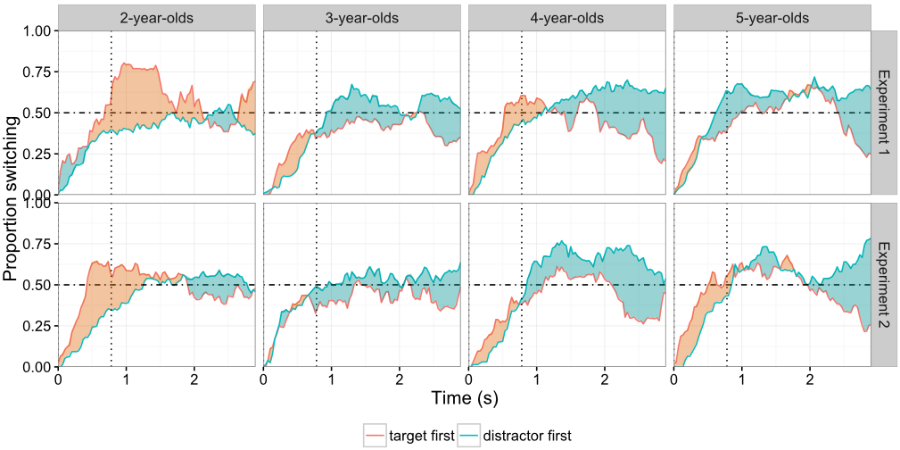
\includegraphics{figs/et_ons-1} 

}

\caption[Onset contingency plot showing results from Experiments 1 and 2]{Onset contingency plot showing results from Experiments 1 and 2. Trials were divided depending on where the participant was first looking: the green line indicates trials in which participants looked at distractor first and made switch to target, and orange line target first and switched to distractor. the size of the green shaded region indicates more switches made from distractor-to-target than target-to-distractor. The size of the orange shaded region represents more switches made from target-to-distractor than distractor-to-target.}\label{fig:et_ons}
\end{figure}
\end{CodeChunk}

One question is whether younger children had difficulty shifting
correctly from distractor to target, or whether they shifted incorrectly
away from target to look at distractor. To explore this question, we
looked at target- and distractor-initial trials separately, contingent
on which item the child was looking toward from the onset of the target
noun (Fernald, Thorpe, \& Marchman, 2010). Top panel in Figure 2 shows
the mean proportion of participants that switched from where they
started in Experiment 1. Thus, increase in shift on distractor-initial
trials is a correct response, whereas increase in shift on
target-initial trials is an \emph{incorrect} response.

Across all age groups, there was an initial increase in shift for both
target-initial and distractor-initial trials, until the offset of the
target word. Then age groups diverged in their looking pattern, and
two-year-olds' struggle was evident: whereas older children's switch to
distractor decreased and switch to target increased, two-year-olds'
switch to distractor continued to \emph{increase} after the target
offset, whereas shift from distractor to target stayed the same.

\section{Experiment 2}\label{experiment-2}

In Experiment 1, we largely replicated Stiller et al. (2015)'s findings
in an eye-tracking paradigm, and showed that adults and older children
(4- to 5-year-olds) look toward the pragmatically felicitous based on
ad-hoc implicature.

But younger children still struggled to look at the inferential target.
Further, 2-year-olds not only did not look at the correct inferential
target, but seemed to look if anything more toward the distractor. A
potential explanation for this pattern comes from the inhibitory demands
of our task. The two items in inference trials differed in salience:
Since the distractor item contained an extra referent (e.g., a carrot
and a banana), it was likely to be more salient. Supporting this idea,
looking to the two-referent item was greater than chance during the
baseline period of each trial. Perhaps 2- and 3-year-olds had difficulty
disengaging from this more salient (and logically possible) distractor
item in favor of the inferentially-correct target item. Inhibitory
control is difficult for children and continues to develop throughout
the period we studied here (e.g., Davidson et al. (2006)). In addition,
several recent studies suggest that inhibitory control might affect word
recognition in similar eye-tracking paradigms (Nordmeyer \& Frank, 2013;
Yurovsky \& Frank, 2015).

Experiment 2 sought to explore the question of whether inhibitory
demands of the task caused younger children's failures. We increased the
saliency of distractor even more by presenting three instead of two
features. If two-year-olds' failures are due to the inhibitory demands,
we predict them to \emph{increase} their incorrect look toward
distractor even more due to its salience. On the other hand, older
children may increase their look toward inferential target, given an
extra feature on the distractor that is negated by the implicature (e.g.
``carrot \emph{but not banana and not cucumber}'').

\subsection{Method}\label{method-1}

\subsubsection{Participants}\label{participants-1}

Participants were recruited as in Experiment 1. A total of 129 children
were recruited but a few were excluded from the sample for the following
reasons: age other than 2 to 5 years (n = 2), parent-reported English
exposure less than our prespecified criterion of 75\% (n = 17),
noncompliance or difficulty with the experimental procedure (n = 1),
experimenter error or technical issues (n = 1). The final sample
consisted of 100 (out of 108 qualifying participants; see Table 1).

\subsubsection{Stimuli}\label{stimuli}

The stimuli were identical to Experiment 1, except for one change:
target items in inference trials and distractor items in control-double
trials now had three features instead of two (see bottom panels in
Figure 1).

\subsubsection{Design and Procedure}\label{design-and-procedure}

The design and procedure were identical to Experiment 1.

\subsection{Results and Discussion}\label{results-and-discussion-1}

As in Experiment 1, participants robustly looked to the targets in the
control trials (Figure 1). Interestingly, age differences were no longer
seen in control-double trials. Importantly, there was no evidence of
performance above \emph{or} below chance for any of the age groups in
inference trials (largest \(t\): \(t\)(28) = 1.78, \(p\) =0.086).

A linear mixed-effects model predicting accuracy based on age and trial
type in Experiment 2 showed a significant main effect of trial type
(\(\beta\) = -0.25, \(p <.001\)), such that looking at target was lower
in inference trials than in control trials. There was no significant
main effect of age or interaction between age and trial type (largest
\(\beta\) = -0.25, \(p >.19\)). Thus, there was no improvement in
looking to the correct target with age increase. As in Experiment 1,
there was no order effect (largest \(\beta\) = 0.09, \(p >.05\)).

A linear mixed-effects model looking at the reaction times of making
first switch from distractors to targets as in Experiment 1, found a
significant main effect of trial type (\(\beta\) = 0.58, \(p <.05\)) and
age (\(\beta\) = -0.1, \(p <.05\)) on the average RT, with no
interaction (\(\beta\) = -0.08, \(p >.23\)). Thus, participants' looking
was faster with increasing age, and looking at inferential targets was
slower and overall lower compared to unambiguous targets, consistent
with what was observed in Experiment 1.

\begin{table}[tb]
\centering
\begin{tabular}{lrrr}
 Predictor & Estimate & Std. Error & $t$ value \\ 
  \hline
Intercept & 0.60 & 0.05 & 12.92 \\ 
  Experiment 2 & 0.07 & 0.07 & 1.00 \\ 
  Control-double & 0.13 & 0.06 & 2.11 \\ 
  Inference & -0.33 & 0.07 & -4.94 \\ 
  Age & 0.04 & 0.01 & 3.34 \\ 
  Experiment 2 * Control-double & 0.02 & 0.08 & 0.25 \\ 
  Experiment 2 * Inference & 0.08 & 0.10 & 0.86 \\ 
  Experiment 2 * Age & -0.02 & 0.02 & -1.28 \\ 
  Control-double * Age & -0.02 & 0.01 & -1.67 \\ 
  Inference * Age & 0.03 & 0.02 & 1.88 \\ 
  Experiment 2 * Control-double * Age & 0.00 & 0.02 & 0.13 \\ 
  Experiment 2 * Inference * Age & -0.02 & 0.02 & -0.79 \\ 
   \hline
\end{tabular}
\caption{Predictor estimates with standard errors and significance information for a linear mixed-effects model predicting accurate looking to target in Experiments 1 and 2.} 
\label{tab:exp2_tab}
\end{table}

\subsubsection{Comparison between Experiment 1 and
2}\label{comparison-between-experiment-1-and-2}

To determine the effect of saliency contrast on children's inferential
processing, we compared looking at targets across both Experiment 1 and
2 for inference trials. A linear mixed-effects model predicting accuracy
based on experiment, age, and trial type (Table 3) revealed significant
main effects of trial type and age, but no interaction between
Experiment 2 and any other variable. Thus, in contrast to our initial
predictions, we did not find evidence of the effect of perceptual
saliency on children's looking patterns. Why did two-year-olds not look
at the distractor more than the target even though the distractor
salience was increased? It is possible that even younger children
benefitted from the strengthed implicature (``carrot \emph{but not
banana and not cucumber}''), or that they simply needed more time to
explore and process all that is displayed.

In both Experiments 1 and 2, we found lower proportion of look toward
inferential target than expected from older children, rarely exceeding
65\%. One possible explanation is that children needed more time to
completely process all the information presented in one trial,
especially for Experiment 2. But based on the current findings,
children, and even adults to some extent, did not reach the predicted
level of referent identification across both Experiments that used
eye-tracking. Thus, this could potentially be a methodological issue:
eye-tracking may not be capturing the full process of implicature
computation. To explore this possibility, Experiment 3 examined
children's implicature computation on another paradigm, using tablet.

\section{Experiment 3}\label{experiment-3}

In Experiment 1, we confirmed that 4- and 5-year-olds reliably looked to
the pragmatically felicitous targets above chance, and thus saw evidence
of their implicature computation. Interestingly, however, the proportion
of looking to target was generally lower than expected, never reaching
beyond 75\%, whereas older children in Stiller et al. (2015)'s paradigm
selected the target much more robustly.

There are a few possible sources of this discrepancy: one potential
source of this discrepancy is the specific type of stimuli used, such as
pictures and utterances. However, the stimuli current paradigm
presumably were easier to process, as we presented two potential
referents instead of three. Yet another important difference is a
methodological one: Stiller et al. (2015) used a behavioral selection
paradigm, whereas we used an eye-tracking procedure. Hence, looking time
in eye-tracking may not be the most accurate measure of children's
selection of the correct target, but eye-tracking does offer the
advantage of looking at the reaction time.

We next wanted use a paradigm that can show both accuracy and reaction
time, to yield comparable data to eye-tracking: tablet paradigm. As
mentioned earlier, a tablet paradigm is a useful, engaging way to
collect data from young children, in that it yields comparable data to
that of naturalistic behavioral paradigms, while making it possible to
examine both accuracy and speed of children's judgments (Frank et al.,
2016). Thus, it can be a more naturalistic and engaging paradigm than
eye-tracking, which requires children to sit still and watch similar
trials repetitively rather than interact with the stimuli. In Experiment
3, we examine children's ad-hoc implicature processing using a tablet
paradigm.

\subsection{Method}\label{method-2}

\subsubsection{Participants}\label{participants-2}

Participants were recruited as in Experiment 1, except that a partial
sample was recruited from a local nursery school. A total of 123
children were recruited but a few were excluded from the sample for the
following reasons: age other than 2 to 5 years (n = 3), parent-reported
English exposure less than our prespecified criterion of 75\% (n = 5),
parental interference (n = 2), noncompliance or difficulty with the
experimental procedure (n = 9). The final sample consisted of 98 (out of
104 qualifying participants; see Table 1)

\subsubsection{Stimuli}\label{stimuli-1}

Items in the visual stimuli used the same set of images as in Experiment
1, presented on a tablet. Same auditory stimuli were used as in
Experiment 1.

\subsubsection{Design}\label{design}

The design was identical to Experiment 2, except that each participant
saw two possible variations of the number of features for each trial
type (2-vs-1 and 3-vs-1 for inference and control-double trials, 1-vs-1
and 2-vs-2 for control-single trials). There were no filler trials.

\subsubsection{Procedure}\label{procedure-1}

An experimenter introduced children to the task using a tablet. Then
they completed two practice trials, where they were asked to select an
obvious, unambiguous referent (e.g., ``cow'' as opposed to ``rabbit''),
followed by 16 test trials.

\subsection{Results and Discussion}\label{results-and-discussion-2}

\begin{CodeChunk}
\begin{figure}[H]

{\centering 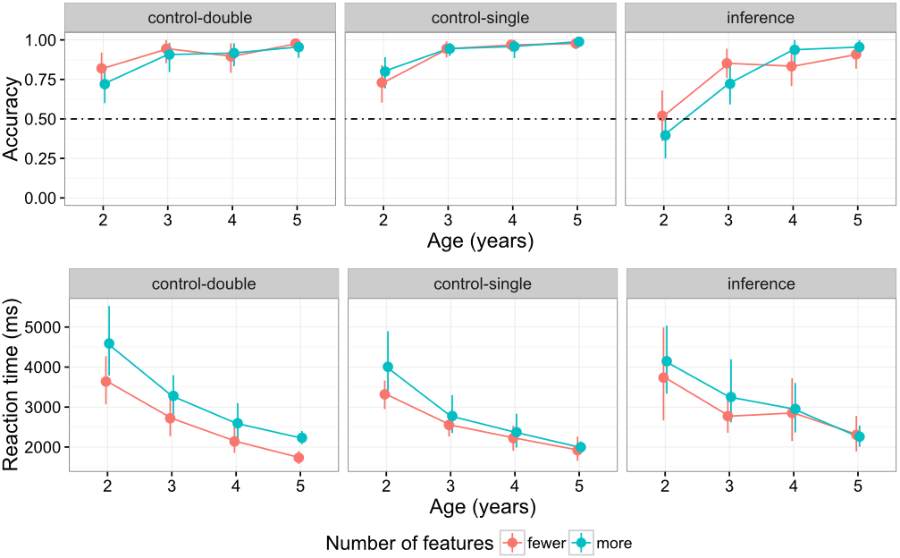
\includegraphics{figs/ipaccrt-1} 

}

\caption[Accuracy rates and reaction times in Experiment 3]{Accuracy rates and reaction times in Experiment 3. Orange lines represent trials in which there were less features present (2-vs-1 for control-double and inference, 1-vs-1 for control-single) and green lines represent trials with more features (3-vs-1 for control-double and inference, 2-vs-2 for control-single).}\label{fig:ipaccrt}
\end{figure}
\end{CodeChunk}

\begin{table}[tb]
\centering
\begin{tabular}{lrrr}
 Predictor & Estimate & Std. Error & $t$ value \\ 
  \hline
Intercept & 0.87 & 0.11 & 8.00 \\ 
  Control-double & -0.07 & 0.14 & -0.48 \\ 
  Inference & -0.01 & 0.15 & -0.08 \\ 
  Age & 0.02 & 0.03 & 0.91 \\ 
  3-vs-1 & 0.05 & 0.14 & 0.33 \\ 
  Control-double * Age & 0.01 & 0.03 & 0.28 \\ 
  Inference * Age & -0.02 & 0.04 & -0.54 \\ 
  Control-double * 3-vs-1 & -0.02 & 0.20 & -0.08 \\ 
  Inference * 3-vs-1 & -0.44 & 0.20 & -2.20 \\ 
  Age * 3-vs-1 & -0.01 & 0.03 & -0.32 \\ 
  Control-double * Age * 3-vs-1 & 0.00 & 0.05 & 0.03 \\ 
  Inference * Age * 3-vs-1 & 0.10 & 0.05 & 2.05 \\ 
   \hline
\end{tabular}
\caption{Predictor estimates with standard errors and significance information for a linear mixed-effects model predicting accurate selection of target in Experiment 3.} 
\label{tab:exp3_tab}
\end{table}

Overall, results in Experiment 3 found more pronounced developmental
gains in both accuracy and speed of ad-hoc implicature processing. All
age groups responded correctly to control trials well above chance, and
all but two-year-olds responded correctly to inference trials (see
Figure 3). Accuracy increased and reaction times decreased with age,
indicating that children become more skilled at implicature computation
as they get older.

A linear mixed-effects model predicting accuracy based on age, trial
type and number of features present showed a significant negative
interaction of inference trial and 3-vs-1 (\(\beta\) = -0.44,
\(p <.05\)), and a significant interaction of inference trial, 3-vs-1,
and age (\(\beta\) = 0.1, \(p <.05\)), indicating that performances on
3-vs-1 inference trials were poorer, especially for the younger
children, two- and three-year-olds. This is in line with our initial
predictions, namely that younger children were expected to have more
difficulty processing implicature when they need to inhibit responding
to the greater perceptual salience of the distractor.

A linear mixed-effects model predicting reaction time based on age,
trial type and number of features present showed a significant main
effect of age (\(\beta\) = -471.34, \(p < .01\)). Thus, children
identified the correct referent faster increasingly with age across all
trial types.

\section{General Discussion}\label{general-discussion}

In the current work, we sought to take a detailed look at children's
ability to compute implicatures, specifically to confirm preschoolers'
ability to compute ad-hoc implicatures, and identify factors that
contribute to children's success and failures as shown in previous
research. Across three experiments, we employed two different
methodologies, eye-tracking and tablet paradigms, to confirm the
developmental trajectories of implicature computation ability, and test
working hypothesis about one potential cause of children's struggle with
implicature: pragmatic-salience tradeoff.

In Experiment 1, we used eye-tracking to replicate previous findings
that children of 4 years and above can compute ad-hoc implicatures.
There were two interesting observations: first, two-year-olds looked
\emph{more} to the distractor than target, rather than look at both
equally, as would be predicted if the looks were based on semantic
ambiguity only. We thus hypothesized that younger children's failures
are due to inhibitory demand of the task: to inhibit look to the more
salient item (distractor; e.g.~plate with a carrot and banana) to look
at the inferential target (e.g.~plate with only a carrot). Second, all
age groups showed lower correct looks to the inferential target than
expected based on previous findings on implicature computation (e.g.
Stiller et al. (2015)). Given that the main discrepancy between the
previous and the current task was methodology -- naturalistic referent
selection paradigm versus eye-tracking -- we wanted to confirm
children's behaviors in tablet paradigm that uses referent selection
task, and examines both accuracy and speed of processing.

Experiments 2 and 3 tested the first question of whether inhibitory
demand drives children's failure to reveal their implicature computation
ability. We found some support for this hypothesis: even though we did
not see any significant differences between trials with less (Experiment
1) vs.~more prominent contrasts (Experiment 2) between inferential
target and distractor in the eye-tracking paradigm, in the tablet
paradigm (Experiment 3), younger children tended to have more difficulty
when distractor was more salient, providing some support for our initial
hypothesis.

Together with previous work on children's implicature computation, the
current work reaffirms that children's pragmatic understanding emerges
early. When cognitive demands are reduced - task is engaging and
naturalistic and alternatives relevant to implicature computation are
available in the context - children as young as 3 years of age
successfully make implicatures, and this ability to process implicatures
accurately and efficiently develops with age.

Consistent with previous findings,younger children (2-year-olds) fail to
compute implicatures in our paradigms, and we successfully identified a
potential cause. Whereas three-year-olds clearly succeeded in our
simplest and most engaging task (Experiment 3), two-year-olds still had
a difficult time choosing the correct inferential target. We found some
supporting evidence of our initial hypothesis that two-year-olds
struggle with the demand to inhibit response to the more salient
alternative to choose the less salient target. Thus, increase in ability
to compute implicatures with age also might be attributed to
developmental gains not only in pragmatic sensitivity but also in
cognitive control. In future work, other ways to amplify the
pragmatic-salience tradeoff and to tease apart the pragmatic
understanding versus cognitive control will be important to identify.

We also found that paradigmatic differences matter in measuring
children's inferential processes. When we compared eye-tracking
(Experiments 1 and 2) versus tablet paradigm (Experiment 3), we found
that children showed more robust inferential target identification in
the tablet paradigm compared to barely-above-chance inferential looking
in the eye-tracking paradigm; developmental gains in the speed of
processing were shown more clearly in the tablet paradigm as well (see
Appendix). Thus, the current work demonstrated the importance of
employing different paradigms to allow complete investigation of
development of an inferential process in question.

In sum, even young children are sensitive to the communicative
intentions behind utterances they hear (Baldwin, 1993; Clark, 2009). Our
work adds to the body of evidence suggesting that by preschool age they
are able to generate sophisticated pragmatic implicatures as well, even
though these inferences are easily masked by other processing demands of
specific contexts and situations. Overall, our current work takes one
step further towards reconciling children's early-emerging communicative
abilities with the complex pattern of successes and failures that they
show in Gricean pragmatics.

\newpage

\section{Appendix}\label{appendix}

\subsection{Subtracting baseline bias in eye-tracking (Experiments 1 and
2)}\label{subtracting-baseline-bias-in-eye-tracking-experiments-1-and-2}

\begin{CodeChunk}
\begin{figure}[H]

{\centering 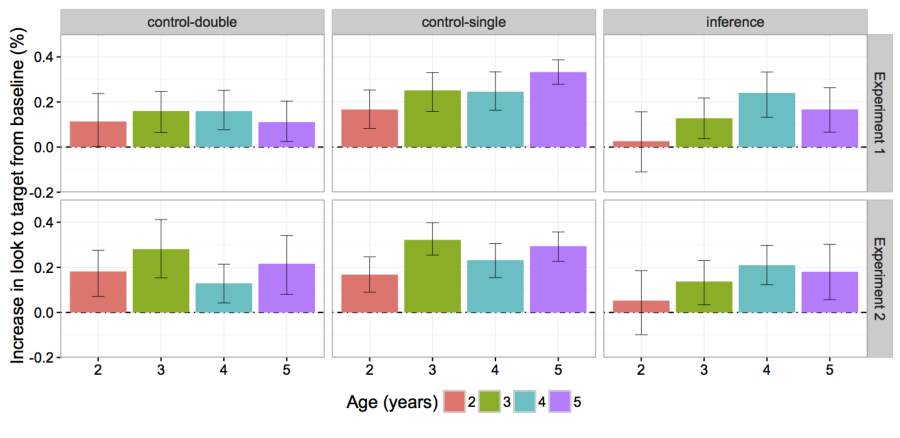
\includegraphics{figs/et_diff-1} 

}

\caption[Increase in look to the target (from the offset of the target noun to 3 seconds after the target noun is produced) compared with baseline looking (from 1 second before the target noun to the start of the target noun)]{Increase in look to the target (from the offset of the target noun to 3 seconds after the target noun is produced) compared with baseline looking (from 1 second before the target noun to the start of the target noun).}\label{fig:et_diff}
\end{figure}
\end{CodeChunk}

In Experiments 1 and 2, while older children (4- and 5-year-olds) looked
to the inferential target above chance, younger children (2-year-olds)
tended to look to the target \emph{below} chance, indicating that they
preferred to look toward the distractor more. This preference toward
distractor was displayed by all age groups before the start of the
target noun in inference trials, which suggested that all children were
initially drawn toward the distractor that was more felicitous, with two
or three features instead of one. Then once the target noun is produced,
participants had to look away from this more felicitous alternative and
direct their attention to pragmatically correct but less felicitous
target.

We hypothesized that the difficulty in inhibiting looks to the more
felicitous item caused younger children's struggle to look to the
correct answer. Supporting this hypothesis, increase in participants'
look to target (computed by subtracting initial baseline looking to
target before start of target noun from look to target after target noun
offset) reveals that, whereas 3- to 5-year-olds increase their look to
the target, 2-year-olds do not show change in attention toward the
target (see Figure 4). Thus, it is possible that 2-year-olds'
identification of the inferential target was hindered by the demand to
inhibit looks to the salient distractor.

\subsection{Comparing across Experiments 1, 2, and
3}\label{comparing-across-experiments-1-2-and-3}

\begin{CodeChunk}
\begin{figure}[H]

{\centering 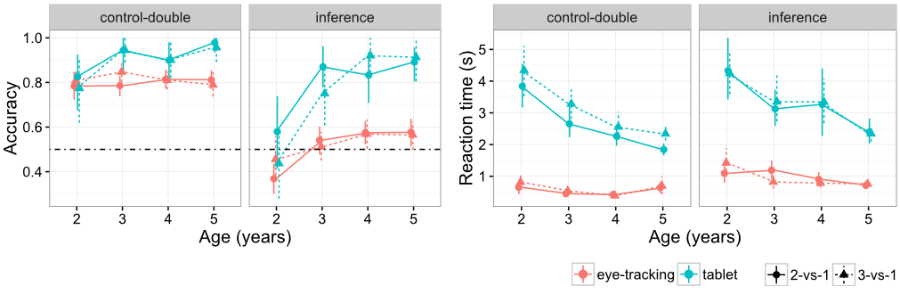
\includegraphics{figs/etip_comp-1} 

}

\caption[Accuracy and reaction times rates for control-double and inference trials (columns) in eye-tracking vs]{Accuracy and reaction times rates for control-double and inference trials (columns) in eye-tracking vs. tablet (iPad) paradigm (colors). Solid lines (circles) represent 2-vs-1 conditions and dashed lines (triangles) represent 3-vs-1 conditions.}\label{fig:etip_comp}
\end{figure}
\end{CodeChunk}

Comparison of accuracy and reaction time measures from the eye-tracking
paradigm (Experiments 1 and 2) and tablet paradigm (Experiment 3) shows
that the developmental trajectory of implicature processing and robust
implicature computation by older children are much more clearly revealed
in the tablet paradigm than in the eye-tracking paradigm (Figure 5). In
fact, accuracy for inferential trials in the tablet paradigm was overall
higher than what was reported in Stiller et al. (2015), possibly due to
visual stimuli that were even more simplified (two referent candidates
instead of three). In the tablet paradigm, both control and inference
trials showed improvement in accurate referent identification over age,
but much more prominently for inference trials. In eye-tracking, the
improvement was observed in inference trials and was much subtler.
Similarly, children responded quicker to the correct referent
increasingly with age in both control and inference trials in the tablet
paradigm, and this gain in efficiency was present in only inference
trials in the eye-tracking paradigm.

\begin{table}[tb]
\centering
\begin{tabular}{lccccc}
 Age bin & Paradigm & M trials (acc) & alpha accuracy & M trials (RT) & alpha RT \\ 
  \hline
2 & eye-tracking & 10.48 & .43 & 3.53 & .45 \\ 
    & tablet & 11.44 & .78 & 15.16 & .29 \\ 
  3 & eye-tracking & 10.44 & .66 & 3.42 & .77 \\ 
    & tablet & 11.55 & .84 & 15.17 & .79 \\ 
  4 & eye-tracking & 10.89 & .61 & 2.87 & -.33 \\ 
    & tablet & 12.00 & .42 & 16.00 & .86 \\ 
  5 & eye-tracking & 10.62 & .57 & 3.55 & -.12 \\ 
    & tablet & 11.84 & .20 & 15.68 & .65 \\ 
   \hline
\end{tabular}
\caption{Standardized reliability coefficients (Cronbach's alpha) for accuracy (acc) and reaction time (RT) by paradigm and age group, along with the mean number of trials for each.} 
\label{tab:etip_rel}
\end{table}

We also examined whether our study measured the variable of interest
with good reliability, by computing Cronbach's \(\alpha\), a statistic
that determines the internal consistency of experimental items (Santos,
1999). Across both eye-tracking and tablet paradigms, Our study
contained three trial types (control-single, control-double, and
inference), with 8, 4, and 4 trials respectively, a small number on
which to compute reliability statistics. We chose to look at 12 control
trials (control-single and control-double) and compute a reliability
coefficient for each experiment and age group, for both accurate looking
and reaction times (see Table 5).

Overall, reliability estimates looks reasonable for accuracy and RT,
with a few aspects to be noted. For accuracy, younger children show
decent reliability in both paradigms, whereas older children show low
reliability for tablet paradigm, which may be due to the ceiling effect
across all trials with tablet. For RT, reliability is generally higher
for tablet paradigms, especially among older children. It should be
noted that RT reliability for eye-tracking was computed with very sparse
data (2-3 trials).

Thus, the tablet paradigm overall more clearly and more reliably showed
children's success in implicature computation compared to eye-tracking.
There are a few different possible interpretations of this result:
eye-tracking may be better at capturing the ambiguity and uncertainty of
ad-hoc implicature. Also, children might have needed more time to
respond for the eye-tracking paradigm.

\newpage

\section*{References}\label{references}
\addcontentsline{toc}{section}{References}

Baldwin, D. A. (1993). Early referential understanding: Infants' ability
to recognize referential acts for what they are. \emph{Developmental
Psychology}, \emph{29}(5), 832.

Barner, D., Brooks, N., \& Bale, A. (2011). Accessing the unsaid: The
role of scalar alternatives in children's pragmatic inference.
\emph{Cognition}, \emph{118}(1), 84--93.

Bates, D., Maechler, M., Bolker, B., Walker, S., \& others. (2014).
Lme4: Linear mixed-effects models using eigen and s4. \emph{R Package
Version}, \emph{1}(7).

Bott, L., \& Noveck, I. A. (2004). Some utterances are underinformative:
The onset and time course of scalar inferences. \emph{Journal of Memory
and Language}, \emph{51}(3), 437--457.

Chierchia, G., Crain, S., Guasti, M. T., Gualmini, A., \& Meroni, L.
(2001). The acquisition of disjunction: Evidence for a grammatical view
of scalar implicatures. In \emph{Proceedings of BUCLD 25} (Vol. 157, p.
168).

Clark, E. V. (2009). \emph{First language acquisition}. Cambridge
University Press.

Davidson, M. C., Amso, D., Anderson, L. C., \& Diamond, A. (2006).
Development of cognitive control and executive functions from 4 to 13
years: Evidence from manipulations of memory, inhibition, and task
switching. \emph{Neuropsychologia}, \emph{44}(11), 2037--2078.

Diamond, A., \& Taylor, C. (1996). Development of an aspect of executive
control: Development of the abilities to remember what I said and to
``do as I say, not as I do''. \emph{Developmental Psychobiology},
\emph{29}, 315--334.

Fenson, L., Dale, P. S., Reznick, J. S., Bates, E., Thal, D. J.,
Pethick, S. J., \ldots{} Stiles, J. (1994). Variability in early
communicative development. \emph{Monographs of the Society for Research
in Child Development}, i--185.

Fernald, A., Thorpe, K., \& Marchman, V. A. (2010). Blue car, red car:
Developing efficiency in online interpretation of adjective--noun
phrases. \emph{Cognitive Psychology}, \emph{60}(3), 190--217.

Fernald, A., Zangl, R., Portillo, A. L., \& Marchman, V. A. (2008).
Looking while listening: Using eye movements to monitor spoken language.
\emph{Developmental Psycholinguistics: On-Line Methods in Children's
Language Processing}, 113--132.

Frank, M. C., \& Goodman, N. D. (2012). Predicting pragmatic reasoning
in language games. \emph{Science}, \emph{336}(6084), 998--998.

Frank, M. C., Sugarman, E., Horowitz, A. C., Lewis, M. L., \& Yurovsky,
D. (2016). Using tablets to collect data from young children.
\emph{Journal of Cognition and Development}, \emph{17}, 1--17.

Grice, H. P. (1975). Logic and conversation. \emph{Syntax and
Semantics}, \emph{3}, 41--58.

Grodner, D. J., Klein, N. M., Carbary, K. M., \& Tanenhaus, M. K.
(2010). ?Some,? And possibly all, scalar inferences are not delayed:
Evidence for immediate pragmatic enrichment. \emph{Cognition},
\emph{116}(1), 42--55.

Gualmini, A., Crain, S., Meroni, L., Chierchia, G., \& Guasti, M. T.
(2001). At the semantics/pragmatics interface in child language. In
\emph{Proceedings of SALT} (Vol. 11, pp. 231--247).

Horn, L. R. (1972). \emph{On the semantic properties of logical
operators in english} (PhD thesis). University of California, Los
Angeles.

Huang, Y. T., \& Snedeker, J. (2009a). Online interpretation of scalar
quantifiers: Insight into the semantics--pragmatics interface.
\emph{Cognitive Psychology}, \emph{58}(3), 376--415.

Huang, Y. T., \& Snedeker, J. (2009b). Semantic meaning and pragmatic
interpretation in 5-year-olds: Evidence from real-time spoken language
comprehension. \emph{Developmental Psychology}, \emph{45}(6), 1723.

Katsos, N., \& Bishop, D. V. (2011). Pragmatic tolerance: Implications
for the acquisition of informativeness and implicature.
\emph{Cognition}, \emph{120}(1), 67--81.

Matthews, D., Butcher, J., Lieven, E., \& Tomasello, M. (2012). Two-and
four-year-olds learn to adapt referring expressions to context: Effects
of distracters and feedback on referential communication. \emph{Topics
in Cognitive Science}, \emph{4}(2), 184--210.

Matthews, D., Lieven, E., Theakston, A., \& Tomasello, M. (2006). The
effect of perceptual availability and prior discourse on young
children's use of referring expressions. \emph{Applied
Psycholinguistics}, \emph{27}(03), 403--422.

Nordmeyer, A. E., \& Frank, M. C. (2013). Measuring the comprehension of
negation in 2-to 4-year-old children. In \emph{Proceedings of the 35th
annual meeting of the cognitive science society}.

Noveck, I. A. (2001). When children are more logical than adults:
Experimental investigations of scalar implicature. \emph{Cognition},
\emph{78}(2), 165--188.

O'Neill, D. K., \& Topolovec, J. C. (2001). Two-year-old children's
sensitivity to the referential (in) efficacy of their own pointing
gestures. \emph{Journal of Child Language}, \emph{28}(1), 1--28.

Papafragou, A., \& Musolino, J. (2003). Scalar implicatures: Experiments
at the semantics--pragmatics interface. \emph{Cognition}, \emph{86}(3),
253--282.

Papafragou, A., \& Tantalou, N. (2004). Children's computation of
implicatures. \emph{Language Acquisition}, \emph{12}(1), 71--82.

Santos, J. (1999). Cronbach\(\backslash\)'s alpha: A tool for assessing
the reliability of scales. \emph{Journal of Extension}, \emph{37}(2),
1--5.

Stiller, A., Goodman, N. D., \& Frank, M. C. (2015). Ad-hoc implicature
in preschool children. \emph{Language Learning and Development}.

Yurovsky, D., \& Frank, M. C. (2015). Beyond naive cue combination:
Salience and social cues in early word learning. \emph{Developmental
Science}.

\bibliography{simpimp.bib}

\end{document}
